\documentclass[a4paper,10pt,review]{elsarticle}

\usepackage{lineno,hyperref} % Use this line to activate reference hyperlinks
% \usepackage{lineno} % Use this line to deactivate reference hyperlinks for ease of reviewing
\modulolinenumbers[5]

% START: Inserted by AJS
\frenchspacing
\usepackage{ifxetex}
\ifxetex
  \usepackage{fontspec}
  \defaultfontfeatures{Ligatures=TeX} % To support LaTeX quoting style
  \setromanfont{Hoefler Text}
  % \setmainfont[Ligatures=TeX]{Palatino}
\else
  \usepackage[T1]{fontenc}
  \usepackage[utf8]{inputenc}
  \usepackage{lmodern}
  \usepackage{textcomp} % directly use the degree (and some other) symbol
\fi

% \usepackage{fixltx2e}
\usepackage[]{graphicx}
\usepackage{wrapfig}
\usepackage{lscape}
\usepackage{rotating}
\usepackage{epstopdf}
\usepackage{ragged2e}  % for '\RaggedRight' macro (allows hyphenation)
\usepackage[pdftex]{color}
\usepackage[margin=2.75cm]{geometry}
\usepackage{upquote}
\usepackage{textgreek}
\usepackage{microtype} % place after fonts; even better typesetting for improved readability
\usepackage{xfrac} % nice fractions
\usepackage{booktabs} % nice tables without vertical lines
\setlength\heavyrulewidth{0.1em}
\setlength\lightrulewidth{0.0625em}
\usepackage[color=yellow, textsize=tiny]{todonotes}
\usepackage[font={small}, labelfont=bf]{caption} % tweaking the captions
\usepackage{gensymb}
\usepackage{amsmath,amssymb}
\usepackage{cleveref} % clever cross referencing figures and tables; last package to include
% END: Inserted by AJS
\usepackage{natbib}

\journal{Progress in Oceanography}

%%%%%%%%%%%%%%%%%%%%%%%
%% Elsevier bibliography styles
%%%%%%%%%%%%%%%%%%%%%%%
%% To change the style, put a % in front of the second line of the current style and
%% remove the % from the second line of the style you would like to use.
%%%%%%%%%%%%%%%%%%%%%%%

%% Numbered
%\bibliographystyle{model1-num-names}

%% Numbered without titles
% \bibliographystyle{model1a-num-names}

%% Harvard
% \bibliographystyle{model2-names.bst}\biboptions{authoryear}

%% Vancouver numbered
%\usepackage{numcompress}\bibliographystyle{model3-num-names}

%% Vancouver name/year
% \usepackage{numcompress}\bibliographystyle{model4-names}\biboptions{authoryear}

%% APA style
% \bibliographystyle{model5-names}\biboptions{authoryear}

%% AMA style
%\usepackage{numcompress}\bibliographystyle{model6-num-names}

%% `Elsevier LaTeX' style
% \bibliographystyle{elsarticle-num}
\bibliographystyle{elsarticle-harv}\biboptions{authoryear}
% \bibliographystyle{elsarticle-num-names}
%%%%%%%%%%%%%%%%%%%%%%%

\begin{document}

\begin{frontmatter}

\title{Predominant air-sea states during coastal marine heatwaves}

%% or include affiliations in footnotes:
\author[firstaddress]{Robert W. Schlegel\corref{mycorrespondingauthor}}
\cortext[mycorrespondingauthor]{Corresponding author}
\ead{3503570@myuwc.ac.za}
\author[secondaddress,thirdaddress,fourthaddress]{Eric C. J. Oliver}
\author[fifthaddress]{Sarah Perkins-Kirkpatrick}
\author[sixthaddress,seventhaddress]{Andries Kruger}
\author[firstaddress]{Albertus J. Smit}
% \author[mysecondaryaddress]{Global Customer Service\corref{mycorrespondingauthor}}

\address[firstaddress]{Department of Biodiversity and Conservation Biology, University of the Western Cape, Private Bag X17, Bellville 7535, South Africa}

\address[secondaddress]{ARC Centre of Excellence for Climate System Science, Australia}

\address[thirdaddress]{Institute for Marine and Antarctic Studies, University of Tasmania, Hobart, Australia}

\address[fourthaddress]{Department of Oceanography, Dalhousie University, Halifax, Nova Scotia, Canada}

\address[fifthaddress]{UWA Oceans Institute and School of Plant Biology, The University of Western Australia, Crawley, 6009 Western Australia, Australia}

\address[sixthaddress]{Climate Service, South African Weather Service, Pretoria, South Africa}

\address[seventhaddress]{Department of Geography, Geoinformatics and Meteorology, Faculty of Natural and Agricultural Sciences, University of Pretoria, South Africa}


\begin{abstract}
As the mean temperatures of the worlds oceans increase, it is predicted that marine heatwaves (MHWs) will occur more frequently and with increased severity however, it is hypothesised that more proximate variables may be responsible for these extreme events. An improved understanding of the mechanisms driving MHWs may allow us to better forecast their occurrence at specific localities. To this end we have utilized atmospheric (ERA-Interim) and oceanic (OISST, AVISO) data to examine the air-sea states around southern Africa during coastal (<400 m from the low water mark; measured \emph{in situ}) MHWs. Nonmetirc multidimensional scaling (NMDS) was used to determine that MHW states were very different from average climatoligcal states. Self-organising maps (SOMs) were used to cluster the MHWs states into 1 of 9 types to determine the predominant patterns. It was found that warm water forced onto the coast via anomalous ocean circulation was the predominant oceanographic pattern during most MHWs. A range of distinct air temperature and wind patterns were found with warm air temperatures over the subcontinent during onshore winds featuring most prominently during MHWs. It may therefore be possible to forecast the occurrence of MHWs when such air and sea states are projected to occur simultaneously. The lack of any strong air-sea patterns during roughly one third of the MHWs implies that sub-meso-scale activity may have been responsible for them and that finer scale observations may be necessary to deduce their physical drivers. These findings motivate for the implementation of local scale real-time \emph{in situ} monitoring of at risk coastal locations in conjunction with the development of a forecasting and disaster prevention system.
\end{abstract}

\begin{keyword}
extreme events \sep coastal \sep atmosphere \sep ocean \sep reanalysis data \sep \emph{in situ} data \sep climate change
\end{keyword}

\end{frontmatter}

\linenumbers

\section{Introduction}
The anthropogenically forced warming of air, land, and sea have been widely publicized over the last several decades both within the literature \citep[e.g.][]{Manabe1967, Sawyer1972, Hansen1981, Cox2000, Rosenzweig2008} and without. Investigations into the negative impacts this warming may have on ecosystems ranges in focus from long term trends \citep[e.g.][]{Scavia2002, Walther2002, Burrows2011} to shifting states \citep[e.g.][]{Travis2003, Grebmeier2006, Blamey2015} to extreme individual events \citep[e.g.][]{Easterling2000, Barrett2008, Wernberg2012a}. Whereas long term temperature trends are projected to have a negative impact on many of earth's systems \citep{IPCC2014}, and the shifts in thermal states brought about by these long term trends are projected to cause irreversible species loss \citep{Thomas2004}, extreme events pose a more immediate threat to ecosystems \citep[e.g.][]{Jolly2005, Denny2009, Hufkens2012}. Extreme thermal events have been given a range of labels but are broadly divided into two categories: cold-spells \citep[e.g.][]{Gunter1941, Lirman2011, Boucek2016} and heatwaves \citep[e.g.][]{Gordon1988, Stott2004, Perkins-Kirkpatrick2016}. We chose here to focus on heatwaves that occur in the sea, classified as 'marine heatwaves' (MHWs).

Several large MHWs, and their ecological impacts, have been well documented. The first of which being a 2003 MHW that negatively impacted as much as 80\% of the Gorgonian fan colonies in the Mediterranean \citep{Garrabou2009}. A 2011 MHW is now known to have caused a permanent ~100 km range contraction of the ecosystem forming kelp species \emph{Ecklonia radiata} in favour of the tropicalisation of reef fishes and seaweed turfs \citep{Wernberg2016} along the southern coast of Western Australia. The damage caused by MHWs is not confined to demersal organisms or coastal ecosystems as demonstrated by a MHW in the North West Atlantic Ocean in 2012 that impacted multiple commercial fisheries \citep{Mills2013}. When extreme enough, such as ``the Blob'' that persisted in the North West Pacific Ocean from 2014 to 2016, a MHW may even negatively impact marine mammals and seabirds \citep{Cavole2016}. Besides increases in mortality due to thermal stress, MHWs may also lead to outbreaks of disease in commercially viable species, such as occurred during the 2015/16 Tasman Sea event \citep{Oliver2017}. 
% Analyses of \emph{in situ} coastal seawater temperature time series from South Africa have shown that MHWs of comparable magnitude to those highlighted here have occurred \citep{Schlegel2017} however, it is not known what damage these events may have caused as little long-term ecological sampling is carried out where these events occurred.

It has been assumed that MHWs should either be caused by oceanic forcing, atmospheric forcing, or a combination of the two however, the scale at which this forcing must occur in order to drive MHWs has yet to be determined. Recent research into the development of a mechanistic understanding between local- \emph{vs.} meso-scale influences on the formation of coastal MHWs has revealed that meso-scale oceanic forcing from offshore onto the nearshore (<400 m from the coast) is far less responsible for the formation of MHWs than hypothesised \citep{Schlegel2017}. It is therefore necessary to consider additional mechanisms that may be responsible for these events. For example, the 2011 Western Australia MHW \citep{Pearce2013} was caused by the aseasonal transport of warm water onto the coast due to a surge of the Leeuwin Current \citep{Feng2013, Benthuysen2014}. Oceanic forcing was also the main contributor of the anomlously warm water during the 2015/16 Tasman MHW when the southward flowing East Australian Current caused a convergence of heat there \citep{Oliver2017}. Conversely, \citet{Garrabou2009} were able to show that atmospheric forcing played a clear role in formation of the 2003 Mediterranean MHW. While more complex, \citet{Chen2015a} also showed that air-sea heat flux could be attributed as the main forcing variable in the 2012 Atlantic MHW. ``The Blob'' however appears to have occurred due to the lack of advection of heat from surface waters into the atmosphere due to anomalously high sea level pressure \citep{Bond2015a}. Outside of these few examples for these well documented events there has been little progress in developing a global understanding of the forcing of MHWs more broadly.

It is now possible to directly compare MHWs occurring anywhere on the globe during any time of year because of a definition developed by \citet{Hobday2016}, which was accompanied by the development of a statistical methodology for calculating these events. Whereas the metrics created for the measurement of MHWs allowed for the comparison of events, they did not directly reveal what may be causing them. Beyond common measurements, it is necessary to identify the possible physical drivers of MHWs so as to be able to compare similar 'types' of events and to be able to move towards a system of prediction.

In order to develop a methodology that could investigate the potential air and/ or sea forcing of multiple coastal MHWs within a single frameework, an index of the mean synoptic air-sea states around southern Africa during the occurrence of these events was created, similar to (RWS: cite Oliver Atlas 2017) for Eastern Tasmania. These states were then clustered with the use of a self-organising map (SOM). The aim of the clustering was to visualise synoptic and/ or meso-scale patterns in the air and/ or sea that occur during MHWs at coastal sites. We hypothesized that i) air and sea patterns would be revealed through clustering; ii) meso-scale patterns would be more distinct in the sea with synoptic patterns more clear in the air; and iii) the air-sea states would aid in the development of a broader mechanistic understanding of the physical drivers of coastal MHWs.

\section{Methods}
\subsection{Study region}
(RWS: Much of the decsription of the study area below could go in the introduction, but I've put it in the methods in the interest of keeping the intro more concise. Additionally, I have left all mention of South Africa (SA) out of the intro in order to make the research less parochial. The results etc. require an understanding of the air and sea around SA, but the focus of the paper should not be the MHWs around SA specifically, but rather that the methodology used here is able to pull out similar synoptic/ meso-scale patterns, regardless of where in the world this work is done.)
The \emph{ca}. 3,100 km long South African coastline provides a natural laboratory for investigations into the forcing of nearshore phenomena as it may be divided into three distinct sections, allowing for a range of meso-scale oceanographic influences to be considered within the same research framework (\Cref{figure1}). The west coast of the country is distinct from the other two as it is bordered by the Benguela Current, which forms an Eastern Boundary Upwelling System (EBUS) \citep{Hutchings2009} when it moves up against the coast. Conversely, the east coast is dominated by the Agulhas Current \citep{Luning1990}, a poleward flowing body of warm water. The south coast is also bordered by the Agulhas current but differs from the east coast in that it experiences both shear-forced and wind-driven upwelling \citep{Lutjeharms2000a} in addition to having significantly more thermal variability than the other two coasts \citep{Schlegel2017}. The range of temperatures experienced along all three coasts are large and the gradient of increasing temperature as one moves from the border of Namibia (site 1) to the border of Mozambique (site 26) is nearly linear. For a more detailed description of the coasts see \citet{Smit2013}.

Air circulation over the study area is dominated by two anticyclonic high pressure cells. The Indian Ocean High sits on the eastern border of the study area and draws warm moist air towards the east coast, whereas the Atlantic Ocean High sits to the west of the subcontinent and draws cool dry air onto the west coast \citep{vanHeerden1998}. Far to the south of the subcontinent, prevailing westerly winds move underneath these two prennial anticyclones \citep{vanHeerden1998}. These three patterns may be seen in \Cref{figure1}. Summer heating may lead to the development of heat lows within the subcontinent, which tend to be absent during winter, allowing for the Indian and Atlantic highs to link over land \citep{vanHeerden1998}. Additionally, the Indian and Atlantic highs, as well as the westerlies, move northwards during winter months, with the effect that the colder westerly winds influence the weather along the south coast \citep{vanHeerden1998}. Air temperatures along the coast are largely influenced by the cold Benguela on the west coast and warm Agulhas current along the east and south coasts.
% These synoptic patterns may be the driving force of wind movement over the subcontinet however, there are meso-scale features, particularly along the coast, that also affect wind movement and air temperature.

The extent of the study area was 10\degree E to 40\degree E and 25\degree S to 40\degree S.

\begin{figure}
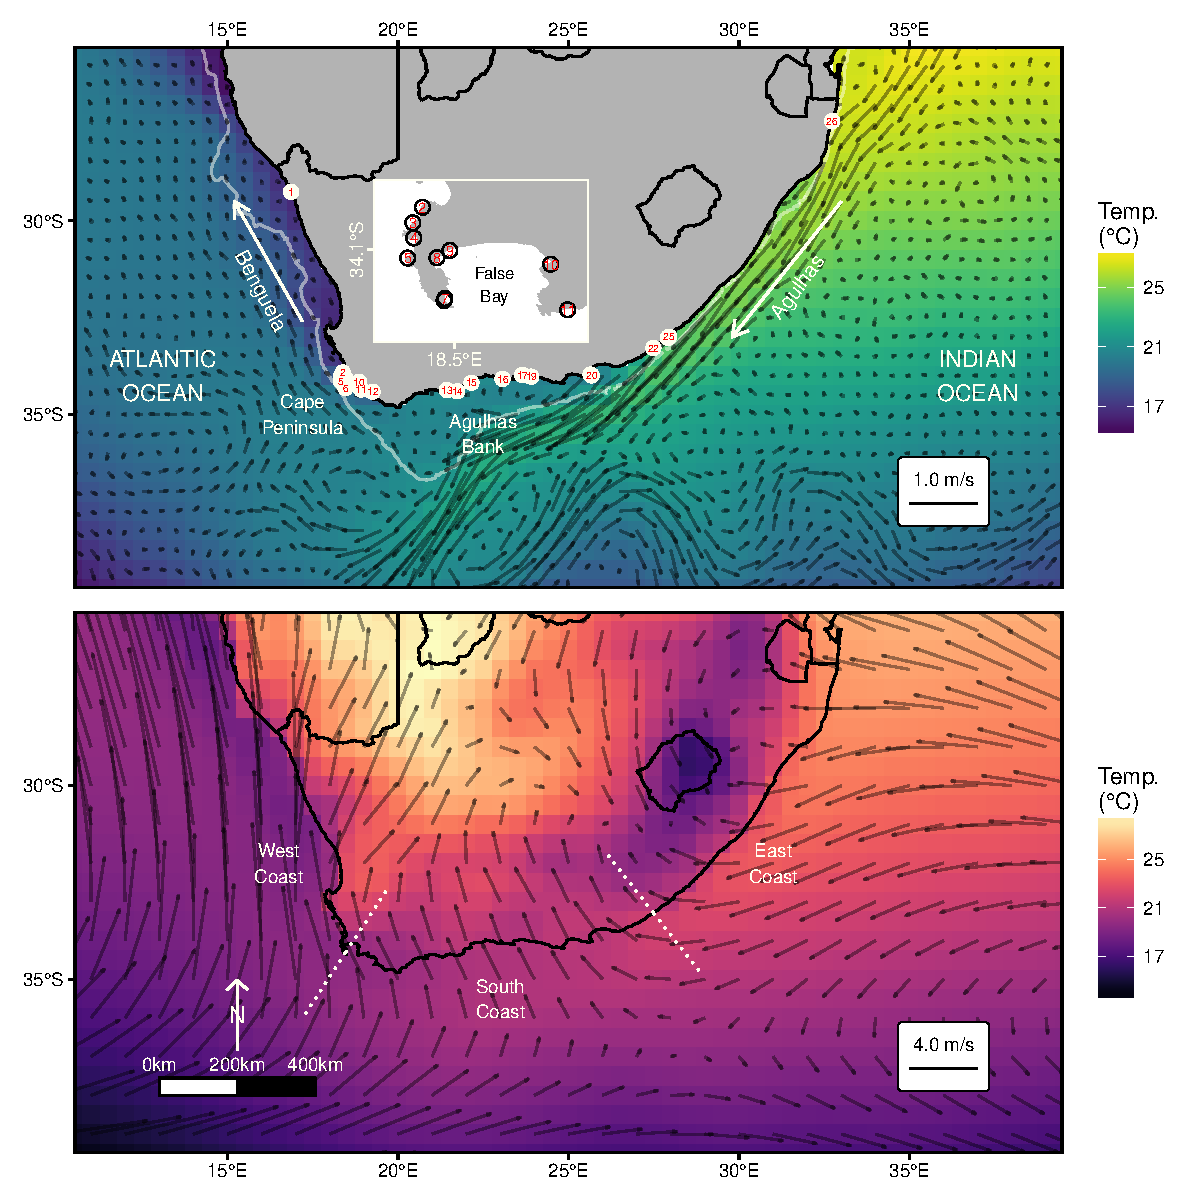
\includegraphics[width=1.0\textwidth]{figure_1.pdf}
\caption{A two panel map of southern Africa. The top panel shows the mean January 15th sea surface temperature (SST) and surface currents from 1993 to 1016, as well as the locations referred to in the text. The locations of \emph{in situ} collection are shown with red numerals over white circles. An inset map of the Cape Peninsula/ False Bay area is shown where site labels are obscured due to overplotting. The bottom panel shows the mean surface air temperature and winds as well as a North arrow, scale bar, and highlights the three coastal sections found within the study area. Note that the temperature and vector scales differ between the two panels. (RWS: Would it be worth including a picture of the mean synoptic air and sea states during Winter, as well? This would be relevant as it would highlight the important atmospheric (anticyclonic) difference between winter and summer. It would be very simple for me to do, but would likely look crowded.)}
\label{figure1}
\end{figure}

\subsection{Data}
\subsubsection{\emph{In situ} data}
The \emph{in situ} coastal seawater temperature data used in this study were acquired from the South African Coastal Temperature Network (SACTN, https://github.com/ajsmit/SACTN, https://robert-schlegel.shinyapps.io/SACTN/). These data are contributed by seven different organizations and are collected \emph{in situ} with a mixture of hand-held alcohol or mercury thermometers as well as digital underwater temperature recorders (UTRs). This data set currently consists of 135 daily time series, with a mean duration of 19.7 years, meaning that many the time series in this dataset are shorter than the 30 year minimum proscribed for the characterisation of marine heatwaves (MHWs, see 'Marine heatwaves' section below) \citep{Hobday2016}. It is however deemed necessary to use these data when investigating extreme events in the nearshore (<400 m from the low tide mark) as satellite derived sea surface temperature (SST) values along the coast have been shown to display large biases \citep{Smit2013} or capture minimum and maximum temperatures poorly \citep{Smale2009, Castillo2010}. Whereas a 30+ year period is ideal for determining a climatology, ten years may serve as an acceptable bottom limit \citep{Schlegel2017}. Following on from the methodology laid out in \citet{Schlegel2017}, time series with more than 10\% missing data or shorter than 10 years in length were excluded from this research. Accounting for these 10 year length and 10\% missing data constraints, the total number of \emph{in situ} time series used in this study was reduced to 26, with a mean length of 22.3 years. The metadata for each SACTN time series used in this study may be downloaded at https://github.com/schrob040/AHW/blob/master/setupParams/SACTN\_site\_list.csv.
% \Cref{tableS1} shows the metadata for the SACTN time series used in this study 
(RWS: I don't think a supplemental section should be given here, rather host everything on GitHub. In fact, should comments like the preceeding sentence be made in the body of the text, or saved for the acknowledgment section? It's a bit jarring to have these long strips of html in the text.)

\subsubsection{Reanalysis data}
To visualise a synoptic view of the air state around southern Africa during coastal MHWs (see sections 'Marine heatwaves' and 'Air-sea state' below) we chose to use ERA-Interim to provide air temperatures (2 m above surface) and wind vectors (10 m above surface) in a single product. ERA-Interim is a comprehensive global atmospheric model that assimilates a wide range of data to create short term forecasts for 60 vertical layers \citep{Dee2011}. These forecasts are then combined with the assimilated data again during each 12-hourly cycle \citep{Dee2011}. ERA-Interim is produced by the European Centre for Medium-Range Weather Forecasts (ECMWF, http://www.ecmwf.int/) and at the time of this writing the chosen variables were available for download from January 1st, 1979 to December 31st, 2016. The data used in this study were downloaded at a daily resolution on a 1/2\degree\~ grid and within the latitude/ longitude of the study region (\Cref{figure1}).

Research on oceanic reanalysis data around southern Africa have shown that none of the products currently available model the complex Agulhas current well \citep{Cooper2014}. It was therefore decided to use remotely sensed data to determine the sea surface temperature (SST) and surface currents in the study area.

\subsubsection{Remotely sensed data}
SST within the study region was determined with the AVHRR-Only Optimum Interpolated Sea Surface Temperature (OISST) dataset produced by NOAA. NOAA OISST is a global 1/4\degree\~ gridded daily SST product that assimilates both remotely sensed and \emph{in situ} sources of data to create a level-4 gap free product \citep{Banzon2016}. These data were averaged to a 1/2\degree\~ grid to match the courser resolution of the ERA-Interim data. At the time of this writing these data were available for download from September 1st, 1981 to June 5th, 2017.

The altimeter products were produced by Ssalto/Duacs and distributed by Aviso, with support from Cnes (http://www.aviso.altimetry.fr/duacs/). Specifically the global 1/4\degree\~ gridded daily surface current product that uses sea level anomaly (SLA) to determine the absolute geostrophic flow of the surface of the ocean. From these absolute flows are derived the U and V vector values that were used in this study. These values were averaged to a 1/2\degree\~ grid to maintain conistent spatial representation between the datasets. At the time of this writing these data were available from January 1st, 1993 to January 6th, 2017.

(RWS: This last paragraph lacks citation because the web portal where these data are available says to cite the data with the following sentence, which I have included as the first sentence in the above paragraph:
The altimeter products were produced by Ssalto/Duacs and distributed by Aviso, with support from Cnes (http://www.aviso.altimetry.fr/duacs/).
Here is a link to where I found this:
https://www.aviso.altimetry.fr/en/data/product-information/citation-and-aviso-products-licence.html)

\subsection{Marine heatwaves}
We use the definition for a MHW given by \citet{Hobday2016} as ``a prolonged discrete anomalously warm water event that can be described by its duration, intensity, rate of evolution, and spatial extent'' as well as the methodology laid out in \citet{Hobday2016} for the analysis of MHWs in this research. The algorithm developed by \citet{Hobday2016} isolates MHWs by first establishing the daily climatologies for a given locality. This is accomplished by finding the range of temperatures for any given day of the year, and then smoothing these daily values further with the use of an 11-day moving window. This produces two values of interest. The first being the average climatology for each day, and the second being the 90th percentile threshold for each day. When the observed temperautres within a time series exceed this threshold it for a number of days it may be classified as a discrete event. \citet{Perkins2013} concluded that the minimum duration for the analysis of atmospheric heatwaves was 3 days whereas \citet{Hobday2016} found that a minimum length of 5 days allowed for more uniform global results for the detection of heatwaves in the ocean. It was also determined that any MHW that had `breaks' below the 90th percentile threshold lasting $\leq$2 days followed by subsequent days above the threshold were considered as one continuous event \citep{Hobday2016}. Previous work by \citet{Schlegel2017} showed that the inclusion of these short 5 day MHWs may lead to spurious connections between events found across different datasets. Therefore we have limited the inclusion of MHWs within this study to those with a duration in the top 10th percentile of all events that occurred within the range of dates available for the reanalysis and remotely sensed data. Thus, from the 976 total MHWs detected in the \emph{in situ} dataset, only 86 were taken.

In order to calculate a MHW it is necessary to supply a climatology against which daily values may be compared. It is proscribed in \citet{Hobday2016} that this period be at least 30 years. Because 20 of the 26 time series used here are below this threshold we have opted to use the first and last complete years of data for each individual time series as the boundaries of the climatological period. Using fewer than 30 years of data to determine a climatology prevents the accurate inclusion of any decadal scale variability \citep{Schlegel2016} however, by using at least 10 years of data we are able to establish a baseline climatology to calculate MHWs \citep{Schlegel2017}. By calculating MHWs against the daily climatologies in this way the amount they differ from their localities may be quantified and compared across time and space. Meaning that this allows researchers to examine events from different variability regimes (i.e. regions of the world) and compare them with a consistent set of MHW metrics. The definitions for the metrics that will be focused on in this paper may be found in \Cref{table1}.

\begin{table}[]
\caption{\small The descriptions for the metrics of MHWs as proposed by \citet{Hobday2016} and adapted from \citet{Schlegel2017}.}
\label{table1}
\centering
\tiny
\begin{tabular}{ll}
\toprule
 Name [unit] & Definition \\
 \midrule
  Count [no. events per year] & \emph{n}: number of MHWs per year \\
  Duration [days] & \emph{D}: Consecutive period of time that temperature exceeds the threshold \\
  Maximum intensity [\degree C] & \emph{i\textsubscript{max}}: highest temperature anomaly value during the MHW \\
  Mean intensity [\degree C] & \emph{i\textsubscript{mean}}: mean temperature anomaly during the MHW \\
  Cumulative intensity [\degree C$\cdot$days] & \emph{i\textsubscript{cum}}: sum of daily intensity anomalies over the duration of the event \\
  Onset rate [\degree C$/$day] & \emph{r\textsubscript{onset}}: daily increase from event onset to maximum intensity \\
  Decline rate [\degree C$/$day] & \emph{r\textsubscript{decline}}: daily decrease from maximum intensity to event end \\
  \bottomrule
  \end{tabular}
\end{table}

The MHWs in the SACTN dataset were calculated via the R package `RmarineHeatWaves', which may be downloaded via CRAN (https://cran.r-project.org/web/packages/RmarineHeatWaves/index.html), with the developmental version available on GitHub (https://github.com/ajsmit/RmarineHeatWaves). The original algorithm used in \citet{Hobday2016} is available for use via python and may be found at https://github.com/ecjoliver/marineHeatWaves.

It is worth emphasising that MHWs as defined here exist against the daily climatologies of the time series in which they are found and not by exceeding an arbitrarily chosen static threshold. Therefore, one may just as likely find a MHW during winter months as summer months. This is a valuable characteristic of this method of investigation because aseasonal warm winter waters may, for example, have deleterious effects on relatively thermophobic species \citep{Wernberg2011}, or aid the recruitment of invasive species \citep{Stachowicz2002}.

\subsection{Air-sea states}
In order to visualise synoptic or meso-scale patterns in the air or sea around southern Africa during a coastal MHW it was necessary to first create daily synoptic images of the air-sea states for all days available across all of the datasets downloaded for this research. The synoptic sea states consisted of SST and surface currents while the air states showed surface air temperatures and surface winds. One mean synoptic air-sea state was then created for each of the 86 MHWs in this study by taking the daily air-sea states during each day during which the event occurred and averaging them together. For example, for a MHW that started on December 1st, 1999, and ended on March 7th, 2000, the 98 daily synoptic air-sea states during that event were averaged to create a single air-sea state that represented the overall pattern that was occurring during that one event. This example may be seen in the top row of panels in \Cref{figure2}. 

The calculation of anomalies required first that a daily climatology be created for the air and sea states. These 366 daily synoptic air-sea climatologies were calculated using the same algorithm used to determine the average daily climatologies for the \emph{in situ} time series, with the climatological period set from 1993 to 2016 as this was the widest period available across all of the gridded datasets. With the average air-sea state known for each calendar day of the year, it was then possible to subtract these daily climatologies from the daily air-sea states during which a MHW was occurring before averaging each individual daily anomaly together to create one mean anomalous air-sea state for each event. An example of the anomalous air-sea states created in this way may be seen in the middle row of \Cref{figure2}.

\begin{figure}
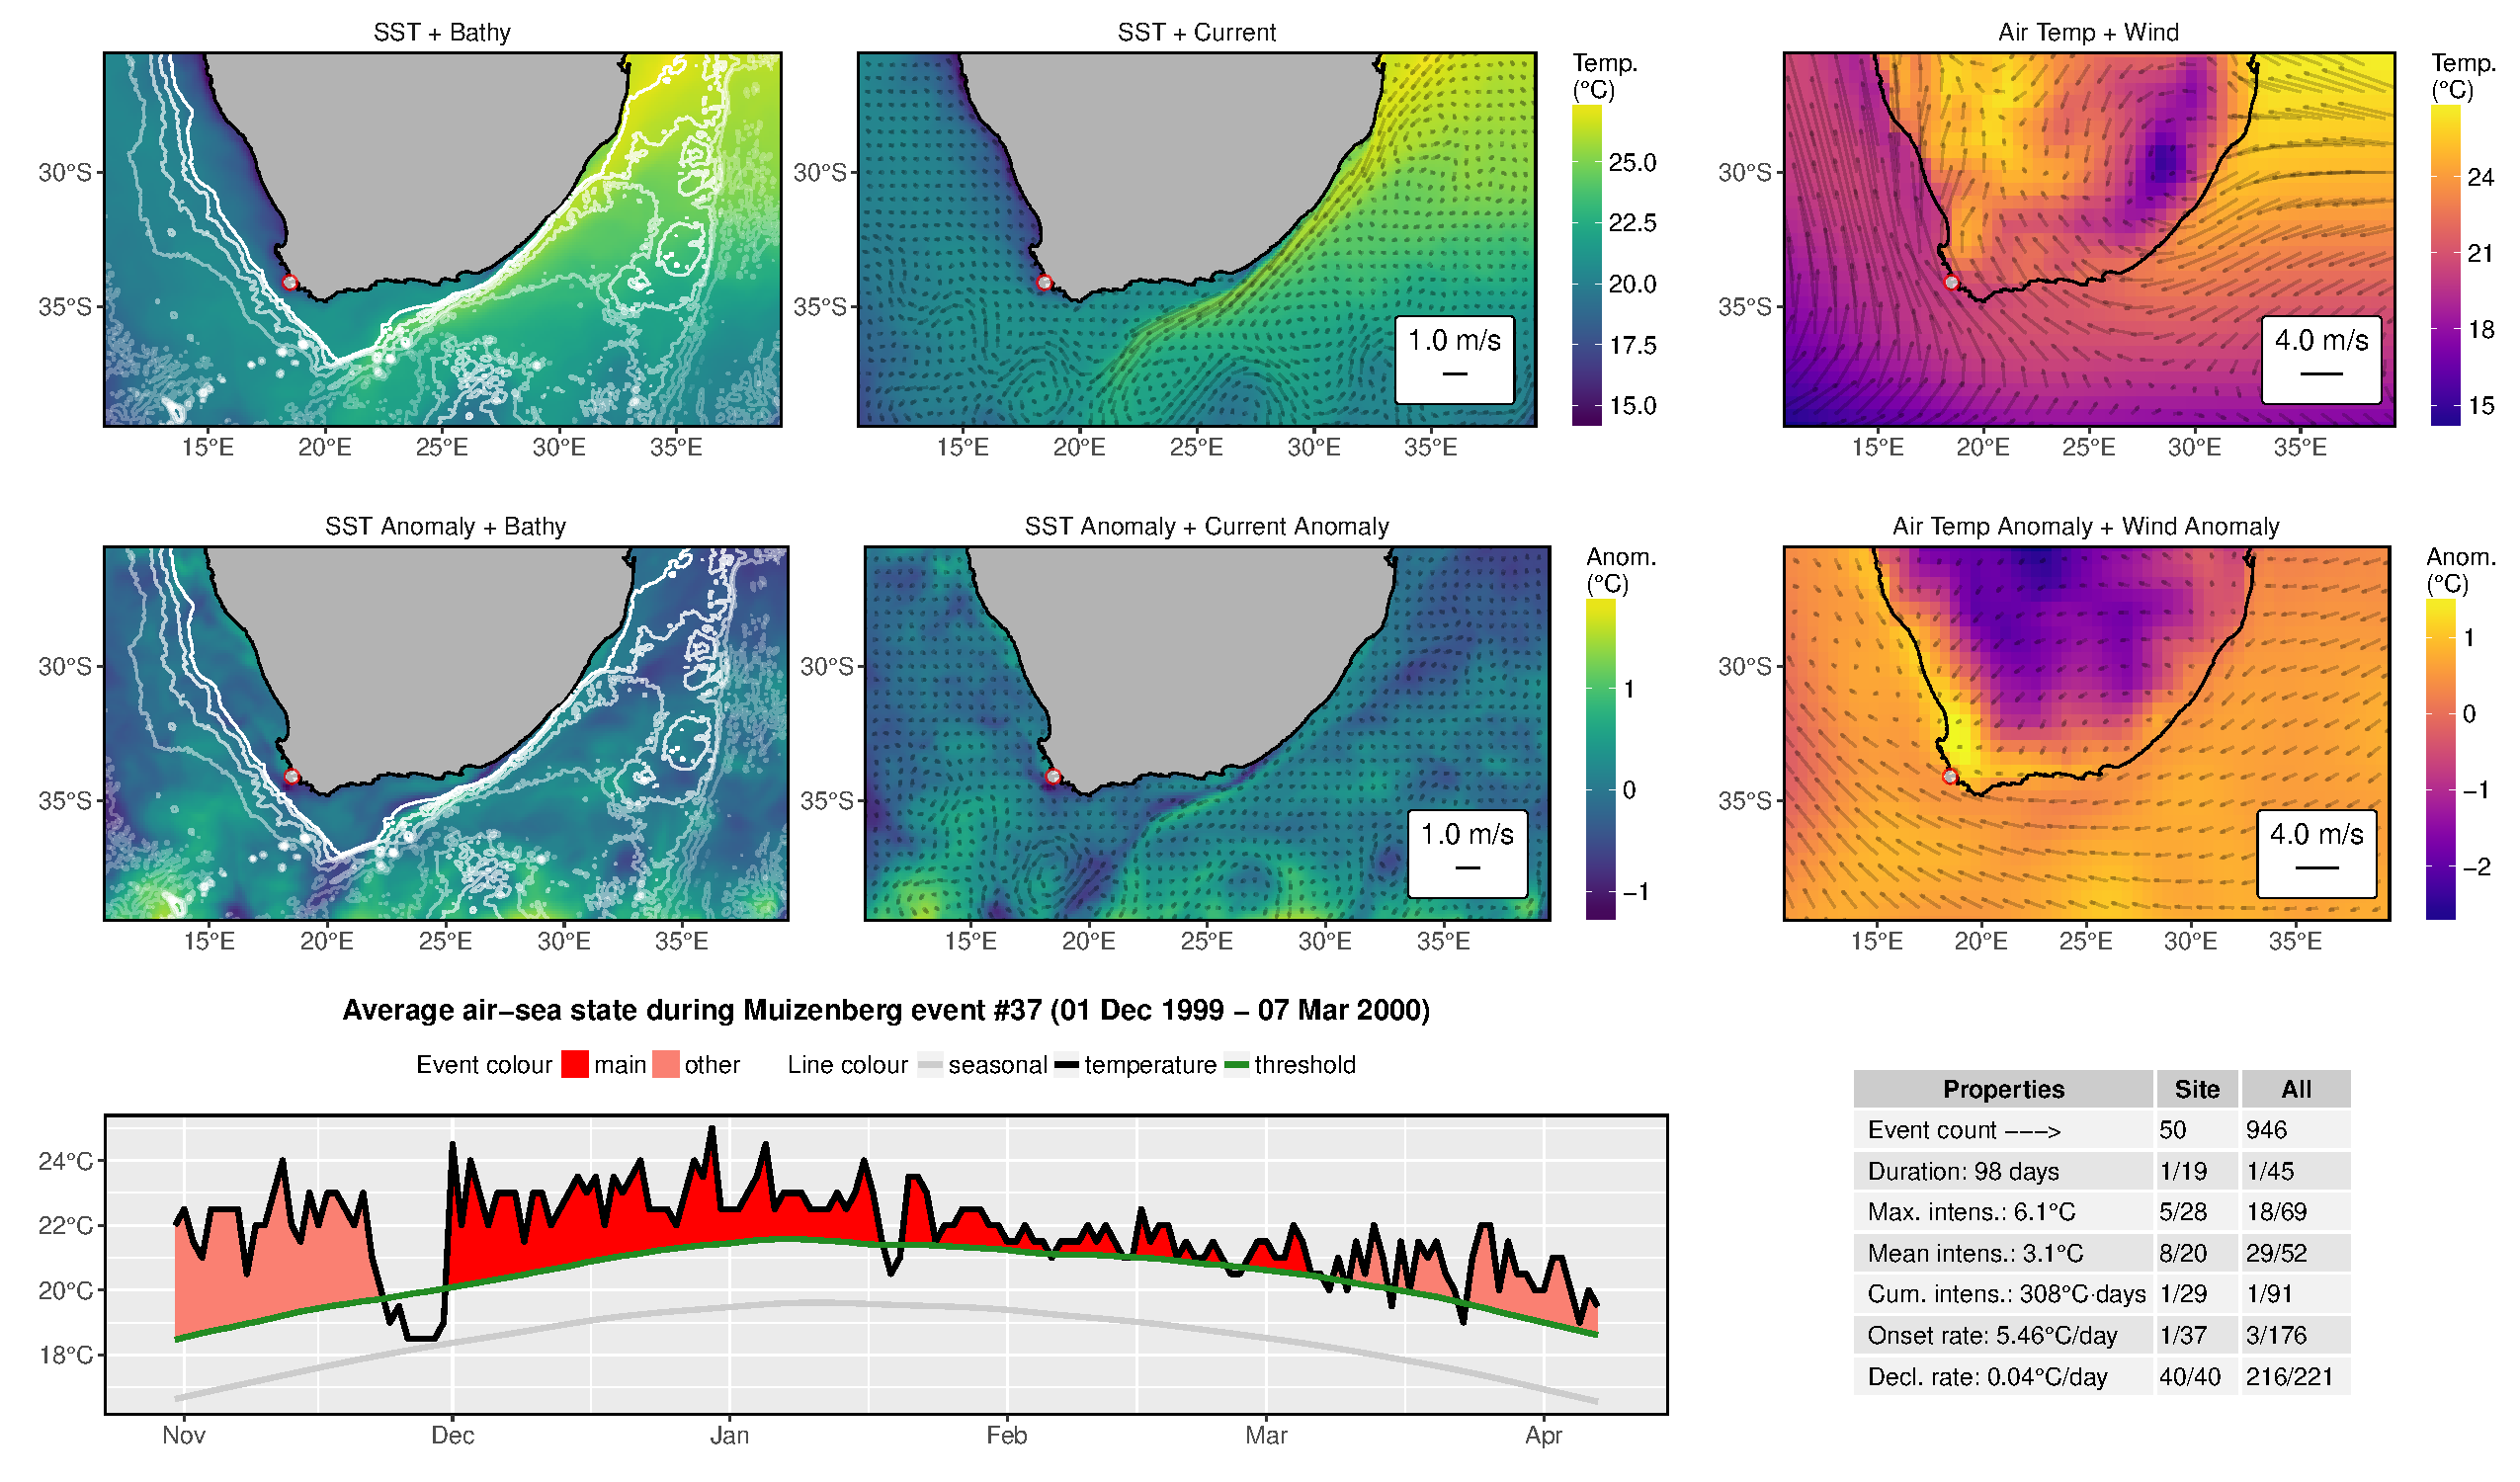
\includegraphics[width=1.0\textwidth]{figure_2.pdf}
\caption{Multiple panelled figure showing a wealth of information for a single coastal marine heatwave (MHW). The location of collection for the \emph{ins situ} coastal seawater temperature time series is shown in each of the top six panels as a white dot with a red border. The top row of panels shows the mean synoptic air and sea states during the MHW, created by averaging all daily air-sea states during the event. The middle row shows anomalies for the mean air and sea states during the event. The mean anomalies were calculated by first subtracting the daily climatologies from the daily values before averaging all of the days together. The left hand panel in the bottom row shows the 'shape' of the MHW and the dates during which it occurred. The table in the bottom left corner shows the values for the relevant metrics of the event as explained in \Cref{table1} as well as their ranking against other events at the same site and all of the MHWs detected along the coast. Similar figures for each of the 86 MHWs used in this study are available here: https://github.com/schrob040/AHW/tree/master/graph/synoptic. 
(RWS: Would it be better to show the anomaly panels in a red-blue scale isntead?)}
\label{figure2}
\end{figure}

\subsection{Nonmetric multidimensional scaling (NMDS)}
% \subsection{Distinction between states}
With the calculation of the 366 daily climatologies for the air-sea states it was possible to determine if the air-sea states during the days in which a MHW was occurring (hereafter MHW states) differed from the average climatology air-sea states (hereafter climatology states). In order to reduce the dimensionality of the air-sea states down to a two-dimensional field to determine the potential relationship between the 86 MHW states and the 366 climatology states, nonmetric multidimensional scaling (NMDS) was used. As it is one of the most robust unconstrained ordination methods available, NMDS is used frequently in ecology \citep{Minchin1987}. Whereas the use of this technique is not wide-spread in climate science, we found that it was effective for reducing the dimensionality of the synoptic air-sea states used here. The temperature, U and V variables that make up each synoptic state, for all MHW and climatology states, were first scaled to a mean of zero within the variance of each variable. These scaled values were then converted into a Euclidean distance matrix before being fed into the NMDS algorithm. An additional benefit of the NMDS algorithm is that it allows for the strength of the influence of categorical variables within the data to be displayed on the resultant bi-plot as vectors. The categorical variables considered when ordinating the MHW and climatology states together were the four seasons during which the day or event occurred/ started, as well as if the value represented a MHW or climatology.

The goal of using NMDS to ordinate the states in this way is not to perform a statistical analysis on the data, but to visualise how each state relates to every other state while simultaneuosly allowing for the effects of the categorical variables on the data to be displayed.

\subsection{Self-organising maps (SOMs)}
Several methods of clustering synoptic data have been employed in climate science. Of these K-means clustering is perhaps most often employed \citep[e.g.][]{Corte-Real1998, Burrough2001, Kumar2011}, with hierarchical cluster analysis (HCA) less so \citep[e.g.][]{Unal2003}. A newer technique, self-organizing maps (SOMs), has been gaining in popularity in climate studies over the past decade \citep[e.g.][]{Cavazos2000, Hewitson2002, Morioka2010}. Here we have used a SOM to cluster the 86 MHW state anomalies.

The initialisation of a SOM is similar to more traditional clustering techniques in that a given number of clusters (hereafter referred to as nodes) are declared by the user before the SOM algorithm randomly assigns each data point into one ofthe nodes. The SOM then iteratively changes the node for each of the data points until the stress within each node, measured as within group sum of squares (WGSS), is reduced as much as possible (cite). Stress here refers to the total variance between data points in each cluster (cite). With large amounts of residual variance meaning the model is fit poorly. SOMs differ from more traditional clustering algorithms in that they also account for the between node stress and endeavour to orient the nodes into the least stressful position possible within a two dimensional space (cite). This allows the user to see not only into which node a given data point (MHW state anomaly) best belongs in, but also what the relationship between the nodes may be (cite). (RWS: Shall more technical details be given here? It may be better to move half of this paragraph up to the previous one.)

The appropriate number of nodes to use in a cluster analysis is well known to be a contentious decision (cite). We have chosen here to use 9 nodes for a number of reasons. The first reason was that SOMs are best run on even grids of data (e.g. 2x3, 3x3, 4x4, etc.) (RWS: cite why even grids are best). Calculating the within group sum of squares (WGSS) value as more nodes were included showed that 4 could be satisfactory, but that at least 6 would be better. Ultimately we settled on 9 nodes as this allowed for a wider variety of different synoptic air-sea states to be separated out from one another, allowing for a better understanding of the dominant air-sea states that exist during coastal MHWs to be formed. It is also recomended by (cite) to allow for the inclusion of at least 10 values within each node.

Because the SOM algorithm was not able to provide consistent results each time the analysis was run, we opted out of using the default random initialization (RI) for the SOM in favour of principal component initialization (PCI). PCI differs from RI in that it uses the two principal components of the dataset, as determined from a principal component analysis (PCA) to initialize the choice of node centres for the SOM (cite). This allows the SOM model to create the exact same result whenever it is run on the same data. (RWS: Should the PCA technique be covered in more detail here?)

Once each MHW state anomaly was clustered into a node a further mean air-sea state anomaly for each node was calculated by taking the average of all of the MHW state anomalies clustered within each node. It was these final mean air-sea state anomalies that were taken as the predominant air-sea patterns during coastal MHWs.

\section{Results}
\subsection{MHW states vs. Normal States}
When we plot MHW states with climatology states on the same two axes of ordination, we see in \Cref{figure3} that the climatology states are all clustered in an elipsoid shape in the centre of the plot, whereas the MHW states are scattered along the top and bottom thirds. Furthermore, the seasons during which the climatology states occurred are clearly important to the ordination of the states but no clear pattern exists for the MHW states. The vectors in \Cref{figure3} show in what direction the categorical variables in the dataset are influencing the placement of each state in the two-dimensional space. We may see that the four vectors for the four seasons each point towards the portion of the elipsoid of climatology states of the same season. We may also see that the vector showing the direction towards which climatology (clim) states are shifted is nearly in the centre of the figure. The vector for the MHW states points in the same direction as the autumn vector, implying that whatever states occurs in autumn may be most similar to states that occur during MHWs.

\begin{figure}
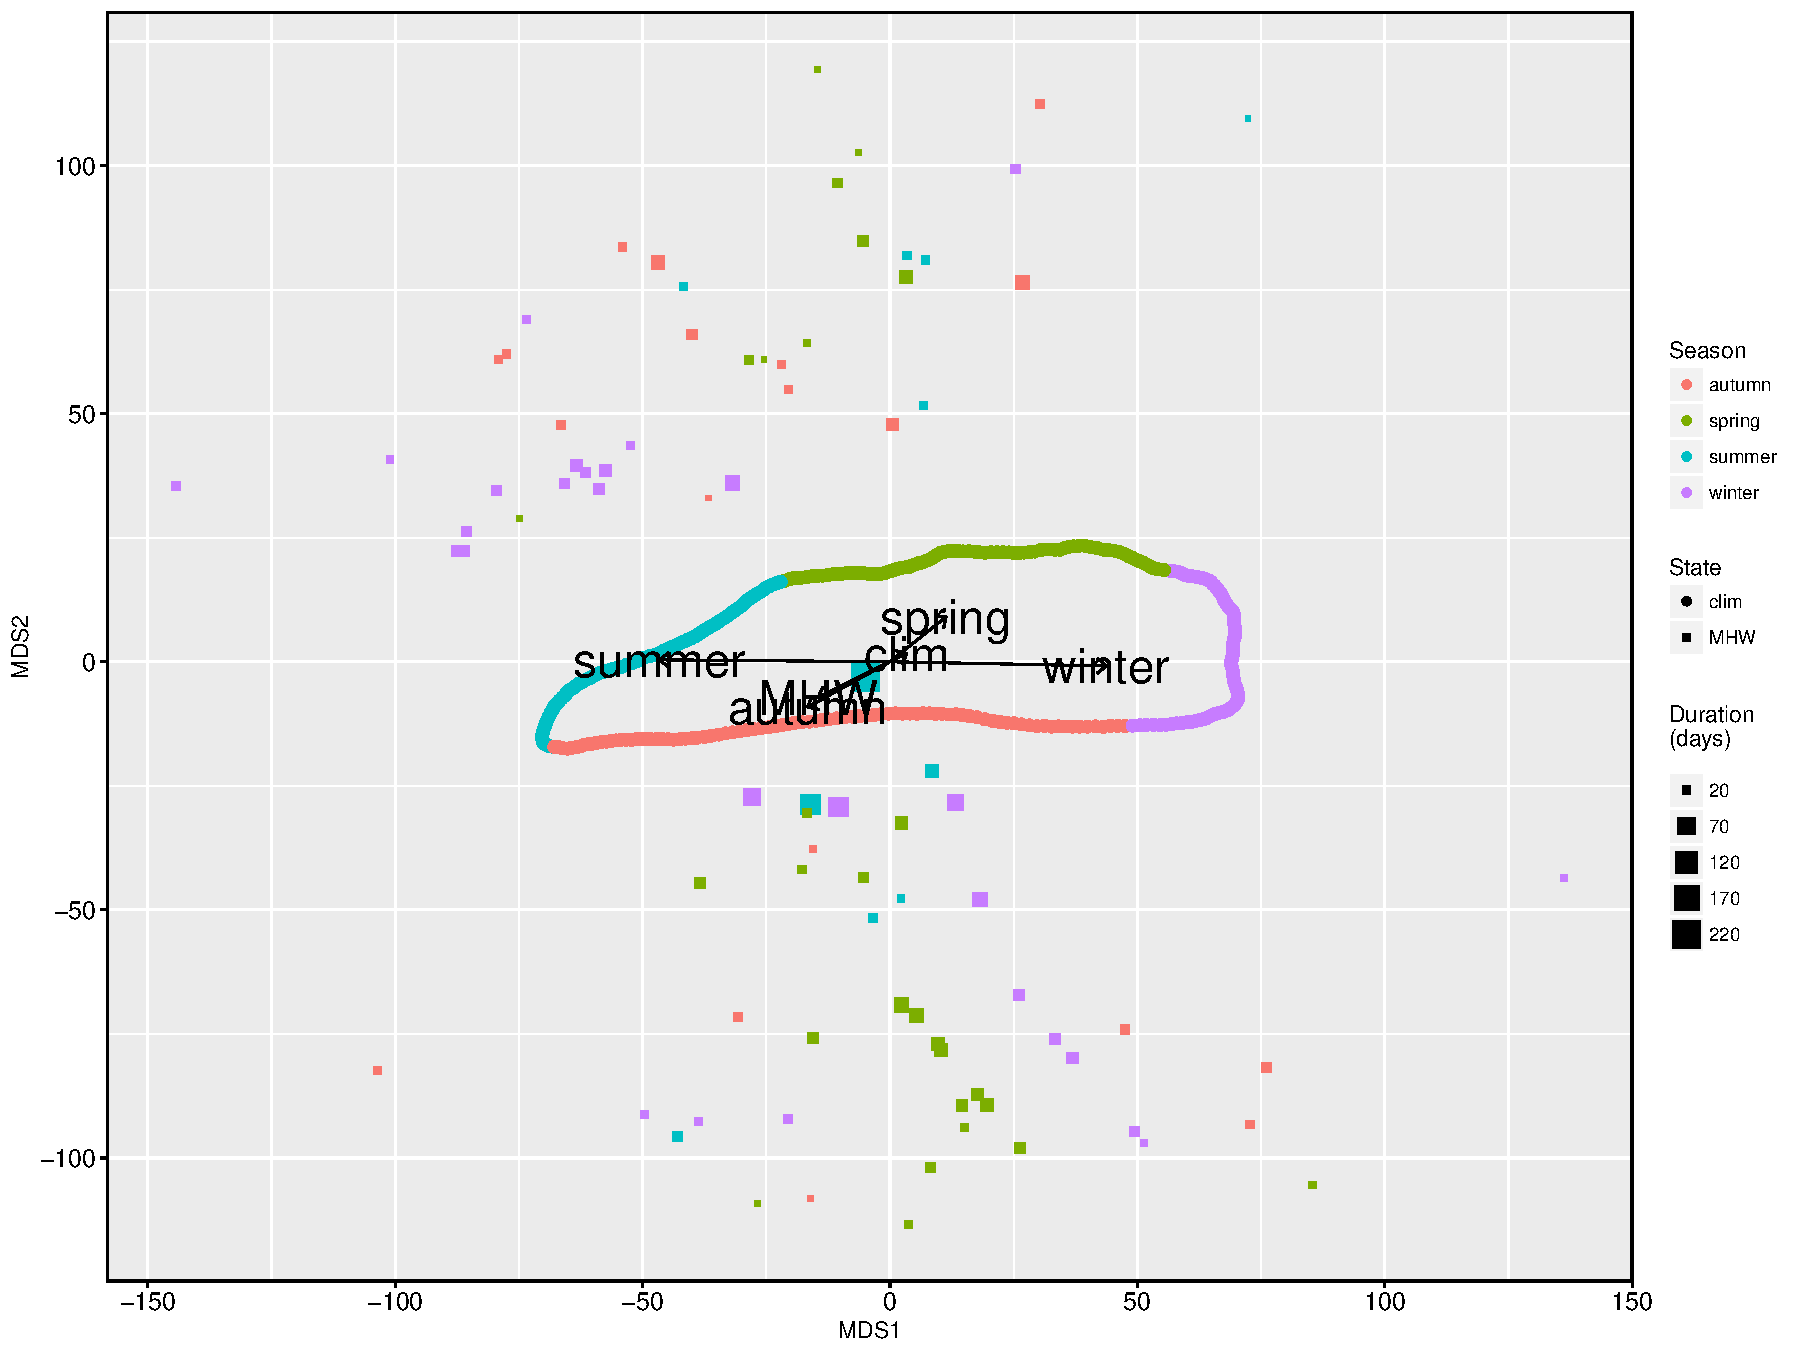
\includegraphics[width=1.0\textwidth]{figure_3.pdf}
\caption{Biplot showing the ordination of climatology states (circles) and marine heatwave (MHW) states (squares). The season of the year durin which the state occurred/ started is shown in colour. The influence of these two categorical vaiables, type of air-sea state and season of occurrence, on the placement of each state in a two-dimensional space are shown as blacl labeled vectors.}
\label{figure3}
\end{figure}

\subsection{MHW patterns}

% (RWS: Consider finding out which pixels are significantly different from the means within the nodes.)
% \subsection{Air-sea states}

The 9 predominant anomalous air-sea patterns around southern Africa during coastal MHWs may be seen in \Cref{figure4}, and the time of their occurrence may be seen \Cref{figure5}. As proposed in \citet{Johnson2013}, the nodes that are output by a SOM should be significantly different from one another to ensure that an excess of nodes has not been used. Using an analysis of similarity we found this to be true for the choice of 9 nodes (p = 0.001).

\begin{figure}
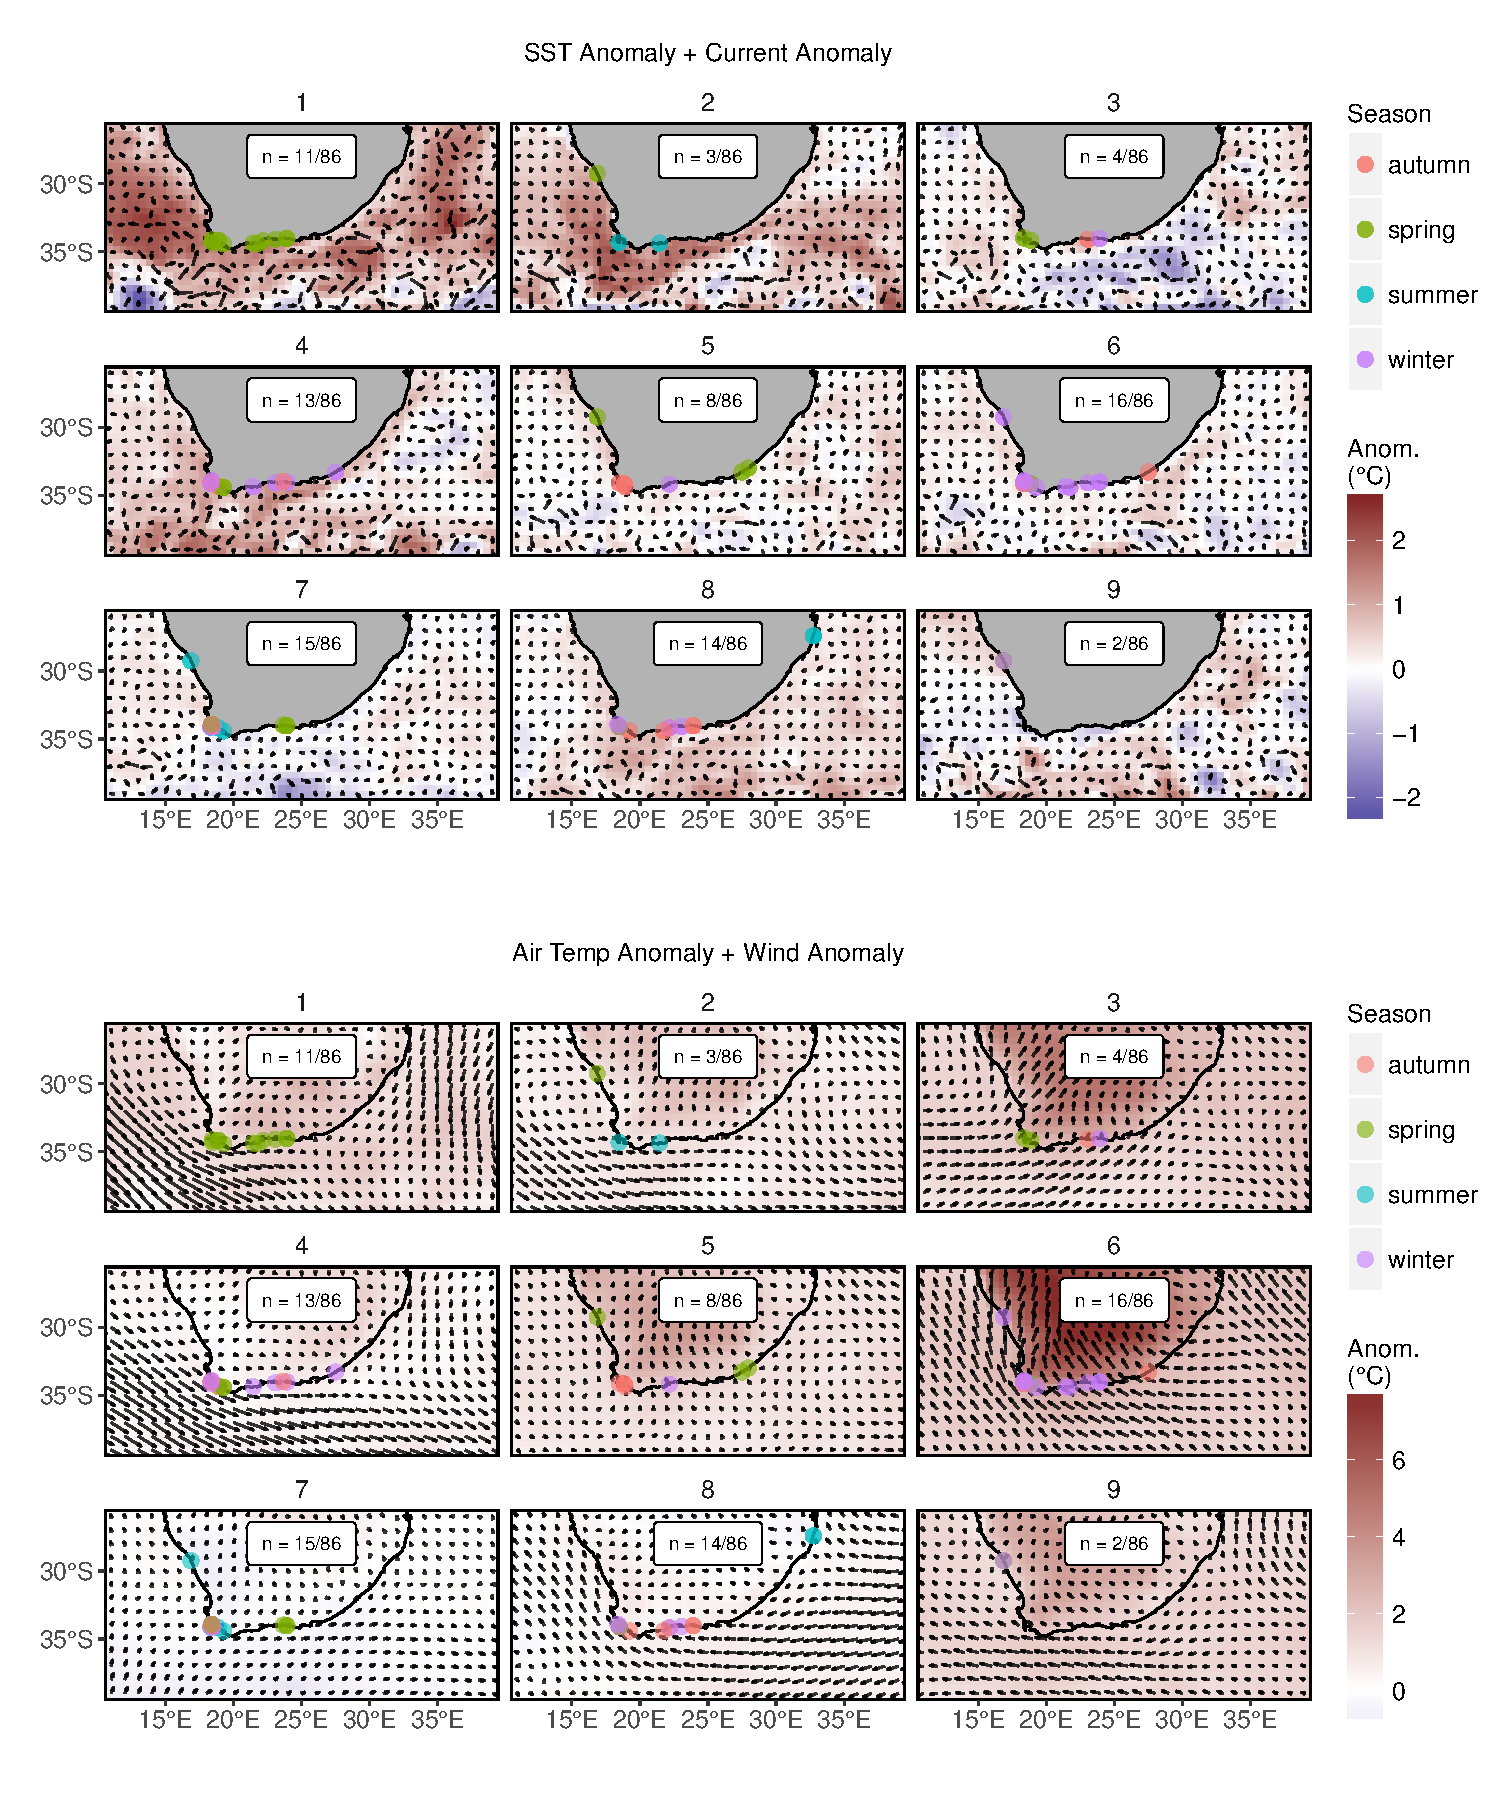
\includegraphics[width=1.0\textwidth]{figure_4.pdf}
\caption{Predominant anomalous air and sea patterns during coastal marine heatwaves (MHWs) as determined by a SOM. The top nine panels show the sea patterns while the bottom nine panels show the air patterns. The current and wind vectors are the same scale as those found in the respective air and sea panels of \Cref{figure1}. The number of events clustered into each node is shown within the white label in the middle of each panel. The location of each coastal MHW within each node is shown with a dot whose colour denotes the season during which that event occurred/ started. Note that the temperature anomaly scales differ for the top and bottom nine panels.}
\label{figure4}
\end{figure}

\begin{figure}
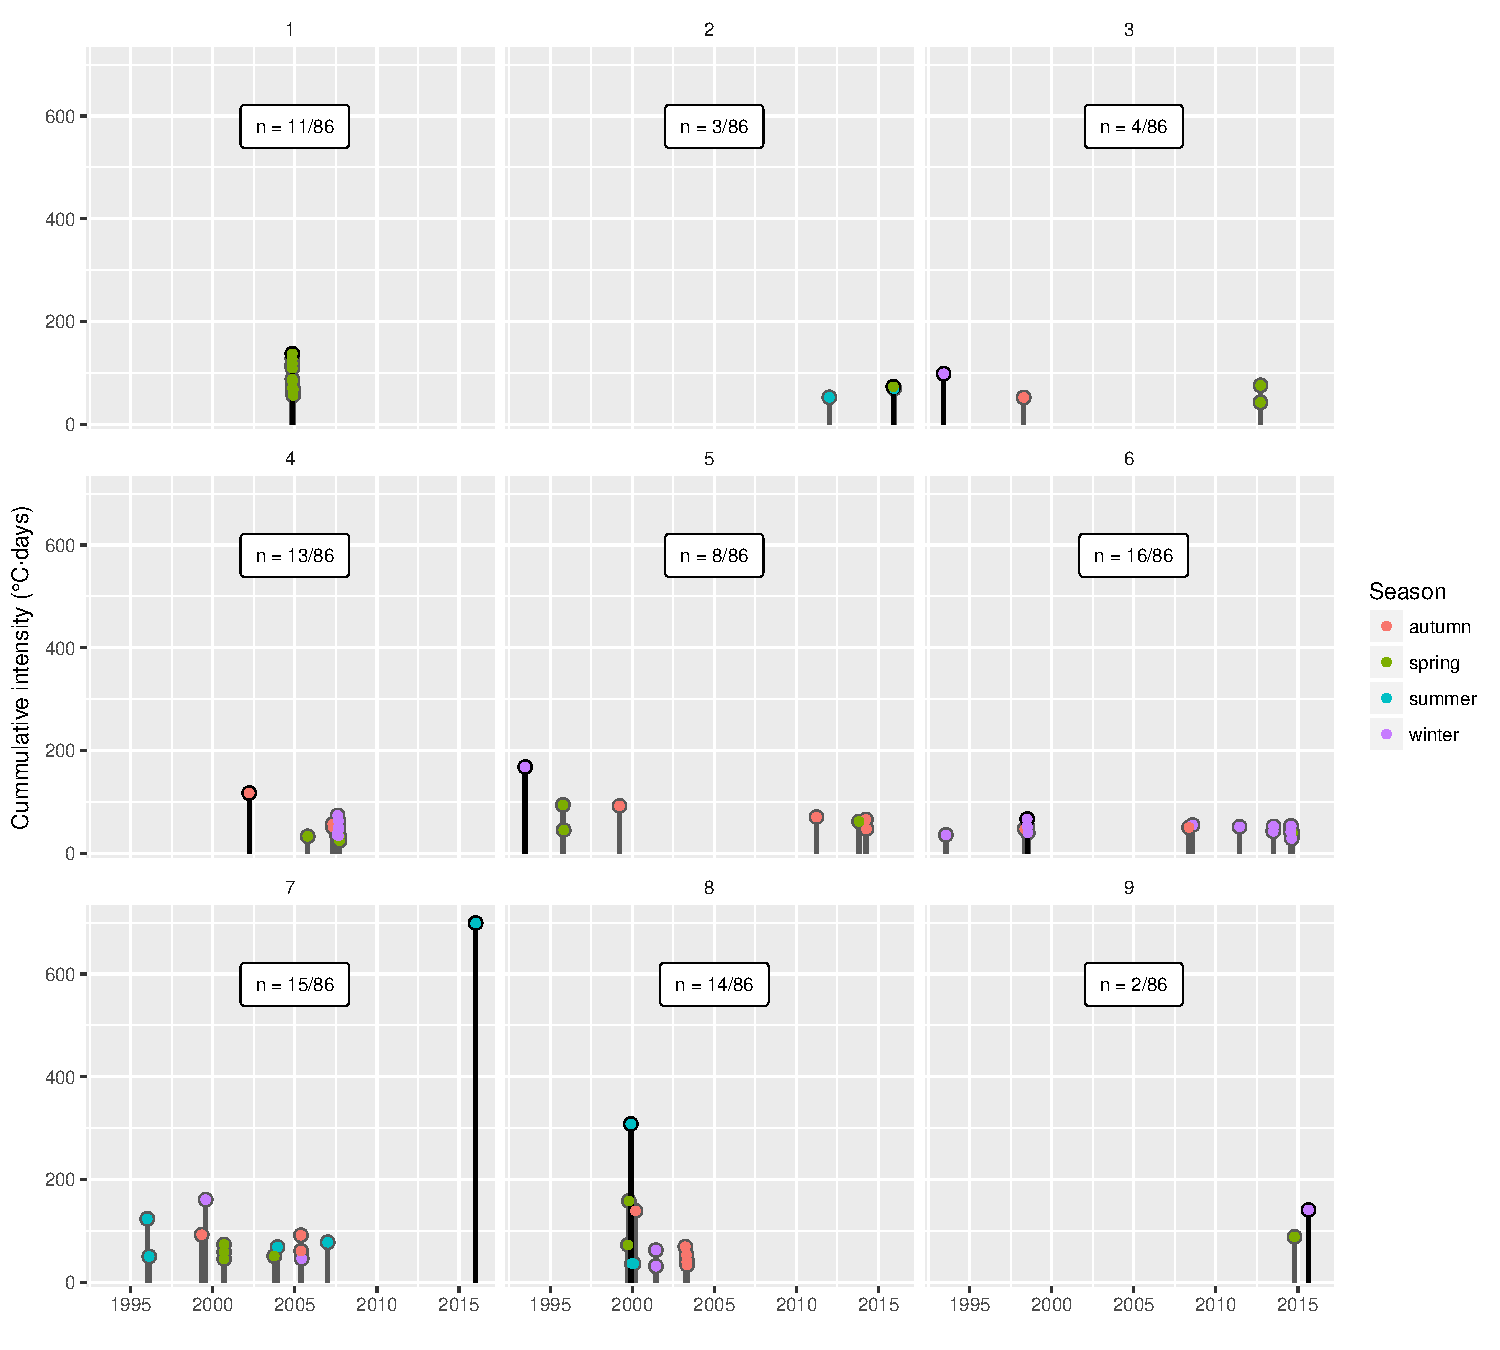
\includegraphics[width=1.0\textwidth]{figure_5.pdf}
\caption{Lolliplots showing the start date for each marine heatwave (MHW) within each node as seen in \Cref{figure4}. The height of each lolli shows the cumulative intensity of the event as outlined in \Cref{table1}.}
\label{figure5}
\end{figure}

\subsubsection{Node 1}
Node 1 in \Cref{figure4} shows the most striking oceanic pattern out of all of the nodes. The mean sea pattern from all of the synoptic sea states clustered into this panel show forcing of the Agulhas current onto the coastal region around the Cape Peninsuala and potentially along the rest of the south coast. The SST anomaly along the coast, as well as in the open ocean is also the warmest of all of the panels. We also see a large strong incursion of the southern ocean in the bottom left of the panel. The air temperature anomaly is mild whereas there are very strong north westerly wind anomalies to the west of the subcontinent and strong northerly wind anomalies to the east. \Cref{figure5} shows that all of these events occurred not only during the same season, but during the same year, too.

\subsubsection{Node 2}
Node 2 shows similar warm SST anomalies in the nearshore along the west and south coasts as node 1. There appears to be some onshore forcing but it is not as strong as in node 1. The air temperature anomalies in this panel are similar to node 1. The wind anomalies are similar to, but weaker than node 1. The Indian and Atlantic highs appear shifted slightly more to the south west.

\subsubsection{Node 3}
Node 3 shows little in the way of strong positive SST anomalies, with much of the water south of the African landmass having negative SST anomalies during the events clustered into this node. There are some atypical surface currents occurring to the south west of the Cape Penisnisula, similar to nodes 2 and 3. The overland air temperature anomalies are strong in this node with the air temperature anomalies over the sea less. The wind anomaly during the events clustered into this node were generally westerleies.

\subsubsection{Node 4}
The events clustered into node 4 show mean sea states with the Agulhas pushing onto the coast and warm SST anomalies along all three coastal sections. The air temperature anomalies were slightly warmer over land than the sea, with neither particularly strong. The wind anomalies were very strong north westerlies.

\subsubsection{Node 5}
Node 5 shows some signs of atypical currents to the south west of the Cape Peninsula but these are not moving towards the coast. The SST anomalies during the events in this node are a mix of warm and cold, with some warm anomalies close to the west and east coasts. The air temperature anomalies were strong during these events, whereas the wind anomalies were not.

\subsubsection{Node 6}
The surface current and SST anomalies in node 6 are similar to node 5, with fewer warm SST anomalies close to the coast. The air temperature anomalies overalnd during these events were in excess of 7\degree C with south easterly wind anomalies. Most of the events in this node occurred during winter months.

\subsubsection{Node 7}
Node 7 shows some atypical currents to the south west but little in the way of onshore forcing of warm SST anomalies. The southern oceanappears to be pushing up into the study area during these events. The air temperatures show a very slight negative anomaly over much of the study area with very weak westerlies winds along the southern poriton of the study area.

(RWS: Look at node 7 in more detail)

\subsubsection{Node 8}
Node 8 shows warm SST anomalies for all but a small portion of the west side of the study area. There is some atypical vorticity to the south of the study area, but this is moving away from the coast. The air temperature anomalies during these events were small and the wwind anomalies were strong south-southeasterlies. 

\subsubsection{Node 9}
The final node shows cold SST anomalies along much of the south coast, with some warm anomalies to the south and atypical vorticity to the south east that does not appear to be reaching the coast. The wind during these events was anomalously strong from the east-southeast with warm air temperature anomalies over the land and sea.

\subsection{Temporal patterns}
MHWs that occurred during summer are only present in three nodes (2, 7, 8) and are the least common, with winter and spring events occurring more than twice as frequently (\Cref{table2}). Most nodes contain MHWs that occurred during at least three seasons and over several years, with the notable exception of nodes 1 and 6 (\Cref{figure5}). All of the MHWs in node 1 occurred during the spring of 2004 within days of one another whereas 13 of the 16 events in node 6 occurred during winter but were spread out from 1993 to 2014.

\begin{table}[ht]
\caption{\small The relevant metrics and statistics for the events found within each node. 
(RWS: Would it be worth adding +- standard deviation to the metric columns?)}
\label{table2}
\centering
\tiny
\begin{tabular}{rrrrrrrrrrrr}
  \toprule
node & count & summer & autumn & winter & spring & west & south & east & duration\_mean & int\_cum\_mean & int\_max\_mean \\ 
  \midrule
  1 &  11 &   0 &   0 &   0 &  11 &   0 &  11 &   0 & 33.50 & 93.73 & 4.04 \\ 
  2 &   3 &   2 &   0 &   0 &   1 &   1 &   2 &   0 & 21.30 & 64.88 & 4.05 \\ 
  3 &   4 &   0 &   1 &   1 &   2 &   1 &   3 &   0 & 25.80 & 67.19 & 3.49 \\ 
  4 &  13 &   0 &   3 &   7 &   3 &   4 &   9 &   0 & 25.20 & 51.07 & 2.89 \\ 
  5 &   8 &   0 &   4 &   1 &   3 &   1 &   6 &   1 & 29.00 & 80.52 & 4.75 \\ 
  6 &  16 &   0 &   2 &  13 &   1 &   5 &  11 &   0 & 23.40 & 47.59 & 2.94 \\ 
  7 &  15 &   6 &   3 &   2 &   4 &   8 &   7 &   0 & 41.10 & 118.55 & 4.21 \\ 
  8 &  14 &   3 &   6 &   3 &   2 &   1 &  11 &   2 & 28.20 & 79.50 & 3.94 \\ 
  9 &   2 &   0 &   0 &   1 &   1 &   2 &   0 &   0 & 46.00 & 114.56 & 4.78 \\ 
  ALL &  86 &  11 &  19 &  28 &  28 &  23 &  60 &   3 & 29.90 & 77.72 & 3.73 \\  
  \bottomrule
  \end{tabular}
\end{table}

\subsection{Spatial patterns}
\Cref{table2} shows that, with the exception of node 1, there are no nodes that contain only events from one coastal section. 8 of the 9 nodes created by the SOM consist of synoptic air-sea states that were occurring during MHWs separated over large distances and by oceanographically dissimilar features. Addionally, only 3 of the 86 MHWs in this study occurred on the east coast.

\subsection{Marine heatwaves}
When we look at the mean statistics for each node (\Cref{table2}) we see that there is a large difference in the mean duration (days) of MHWs clustered therein. Nodes 4 and 5 show the longest mean durations however, the mean duration in node 5 is skewed by having one very long event and only two total events in that node. Nodes 9 and 2 are characterized by having the shortest MHWs. As large cumulative mean intensities are generally a product of lengthy MHWs, it is not surprising to see that Nodes 4 and 5 also have the highest values for this metric as well. Again though node 5 is misrepresented in this regard due to the one large event clustered there. As for the maximum intensity of events within each node, there is less difference between the nodes than for the other two metrics shown. Nodes 2 and 8 however did have events with the lowest maximum intensities (\degree C) on average.

\section{Discussion}


(RWS: Atmosphere notes:
Summer months more pressure from the anticyclones, winter months more pressure from the south.
Constant pressure cells near the surface: South Atlantic Anticyclone, South Indian Anticyclone, East Pacific Anticyclone.
The movement of these cells over the continent largely control weather and climate.
Also low pressure cell to the North. This deminishes in winter, lessening chances for rainfall inland. THis then shifts rainfall south onto the coast. Tyson and Preston-Whyte (2000)
During July the ITCZ is located over northern Africa, so that southern Africa does not benefit from the convective activity and the resulting atmospheric moisture generated by it at that time of the year. During January however, which is quite representative of summer, the situation is quite different.
Hurry and van Heerden (1986) for the general patterns during summer.
Many factors can play a role in the wind speed and direction on the local scale along the coast e. g. topography, ones actual distance from the coastline, as well as the land-sea boundary (Hsu, 1988)
)


\subsection{MHW states vs. Normal States}
(RWS: Talk more about how the event days cluster out differently from normal days.)
As one may see from the flat ellipse of multi-coloured circles in \Cref{figure3} (the daily climatology points), the variance represented in the x axis is seasonality. 
% Indeed, if the dates are included in the figure above they are in a nearly contiguous state. With January 1st in the top left edge of the ellipse of blue squares with the dates then moving clockwise. May is roughly in the middle of the top of the ellipse and October in the middle on the bottom. 
The air-sea states during MHWs appear to be controlled by the variance represented by the y axis. This then must be some sort of variance that is aseasonal. Likely the anomalous characteristics of air and or sea that occur during the events. This shows that whatever those states may be, they are independent from the common air-sea states that occur at any time during the year. Also worth noting is that the daily climatologies for summer and winter do not cluster at all with any of the events (\Cref{figure3}). They are almost all clustered with autumn, and a few with spring days.

\subsection{MHW patterns}
Immediately apparent in the clustering of the data is that node 1 stands out in starkest contrast to the other nodes the most anomalously warm air and sea states as well as having the strongest winds and currents. As one moves from the right hand nodes to the left they become progressively less intense. With less and less of a pattern present. These left hand nodes serve to show that there are still many coastal MHWs that occur without any strong meso-scale pattern on average. Or at least not a pattern that has occurred often enough over the past 30+ years that would afford them their own node. Due to the vast dissimilarity between the 9 nodes, only 2 events were clustered into the central node. Otherwise the clustering of events into nodes was equitable. Also important to note is that a common pattern in many of the nodes, but particularly node 6, is the abnormal retroflection of the Agulhas current onto the Agulhas Bank (\Cref{figure4}).

If we look at the events within the nodes via lolliplots (\Cref{figure5}) we see that only one of the nodes shows an air-sea state during primarily one large event that was recorded at multiple locations (node 6). Besides node 6 (and 5), the other nodes consist of a medley of multiple independent events that occurred during different years and seasons, and of varying magnitudes, that cluster together due to their similarity. These nodes represent what a more common air-sea state during a coastal MHW may look like.

\citet{Schaeffer2017} Sub surface MHWs

\citet{Beal2011} Agulhas leakage likely to increase. This is associated with interglacial periods. Whereas the abatement of leakage is associated with severe glacial periods. This is all due to the north or southward shift of westerly winds over the Atlantic.

% \subsection{MHW patterns}
Most notable from the clustering of these events has been the Agulhas current retroflecting (RWS: Talk about Agulhas Leakage instead) north towards the Cape Peninsula, rather than its usual southward retroflection (cite), when many coastal MHWs were detected. When the Agulhas retroflects north it leads to Agulhas leakage, where warm Indian Ocean water bursts into the colder Atlantic Ocean (cite). These warm eddies then typically spin up along the west coast. This transport of a large body ofg atypically warm water along a large stretch of coastline is a similar finding to the cause of the Western Australia MHW in 2011 where an unusual surge of the Leeuwin Current forced a large body of anomalously warm water onto the coast \citep{Feng2013, Benthuysen2014}. This onshore forcing of water is most apparent in node 1 (\Cref{figure4}) however, nodes 2, 3 and 4 show a similar though less pronounced oceanic pattern, meaning that roughly one third of the events in this study have occurred during Agulhas leakage. Node 8 also shows onshore forcing of the Agulhas current, but with no large leakage into the Atlantic Ocean. Taken together with the events that occurred during Agulhas Leakage, over half of the longest events detected have occurred during some sort of anomolous Agulhas behaviour. This is strong support for the relationship between the Agulhas current and coastal MHWs. As the Agulhas current becomes more variable and oscilates over a wider distance (cite) this may mean that more MHWs will be occurring along the south and west coasts.

With the exception of nodes 4, 7, and 8, all of the atmospheric states during coastal MHWs showed warm air temperature anomalies. The largest of these anomalies occurred in node 6, with overland temperature anomalies in excess of 7\degree\ C. It is also worth noting that the anomalies overland are genrally greater than over the sea when the vents were occurring for almost every node. There were also only two main wind patterns during coastal MHWs. Nodes 1, 2, 3, and 4 show strong northwesterly to westerly anomalies. Nodes 

From this one must infer that air temperatures will almost always be anomalously warm during a coastal MHW and that winds will usually either be anomolously strong from the northwest or south east. Furthermore, the nodes with the greatest overland air temperature anomalies (nodes 3, 5, 6, and 9) also show an overall greater proportion of cold than warm SST anomlies as well as onshore wind anomalies. This implies that the MHWs in these nodes were forced by the onshore winds occurring during warm atmospheric anomalies and and not by oceanic conditions. These nodes account for roughly one third of the events in this study.

The lack of a strong air or sea pattern in node 7 implies that the 15 events that were clustered there do not share any common pattern. Meaning that there may still be many MHWs that occurr not because of any predominant air or sea pattern. This is an important finding as it shows that even though clear patterns in air and sea may exist during most MHWs, these events may still occur during entirely novel conditions.

\subsection{Temporal paterns}
With the exception of node 6, all of the nodes produced by the SOM contain events not only over large periods of time, but during most if not all four seasons of the year. This means that the meso-scale drivers of MHWs are truly aseasonal. Indeed, as we may see in \Cref{figure3}, not only do events occurring during a particular season not relate to the air-sea states during that season, they do not relate to air-sea states during any time of the year. The only small exception to this finding being that some small similarities may be noted during some days in spring and several more during autumn. This implies that whereas air-sea states during events depart from anything seen throughout a normal year, they most closely resemble air-sea states during the tumultuous transitional seasons of spring and Autumn (cite?). (RWS: Calculate the difference in variance between the seasons.)

Also of interest in this study was during which season do MHWs in excess of 15 days tend to occur. We found, to some surprise, that only a small portion (\Cref{table2}) of MHWs occurred during summer months. This implies that the phenomena that may be driving these long MHWs occur more often during the cooler months of the year. This may mean that summer months around southern Africa are more stable than at other times of the year, or that the processes that drive long MHWs are linked to the transitioning of warmer temperatures to cooler temperatures. And vice versa. It is not possible to draw any conclusions on this relationship from the output of this research. Further investigation into this possible causal link is required. (RWS: Rather look for cases in the literature in which stable states occur during winter months that could argue for this observation.)

\subsection{Spatial patterns}
That 8 of the 9 nodes created by the SOM consist of synoptic air-sea states that occurred during MHWs on different coastal sections of the study area leads to two possible implications. (RWS: Rewrite this sentence if you don't simply remove this subsection instead.) The first is that the onshore forcing of the Agulhas current during thee MHWs must be extending onto the shore through the Benguela upwelling system. The other implication is that it may be temperature exchange between air and sea at the coast that is leading to these events. (RWS: Must expound upon these two ideas more fully.)

Therefore it is difficult to judge any potential relationships between synoptic patterns that may be responsible for events only on the east coast, or between the east coast and other sections of the coastline.

\subsection{Marine heatwaves}

% \subsection{Normal days}
% Move the above two sections here.

\section{Conclusion}

(RWS: Talk about potential for prediction, but issues with reanalysis data)

(RWS: Link to EKE studies)

This research has highlighted that coastal MHWs with durations in the 10th percentile often occur during the abnormal advection of water onto the coast due to atypical meso-scale activity. In the case of the west and south coast sections of South Africa this offshore water is often warmer than coastal waters and so it was not necessary that the offshore waters be aseasonally warm at their point of origin. Anomalous wind and air temperature patterns during coastal MHWs were found to cover a wide range of states and so no one pattern shows a clear relationship to these events.

It was also found that the average synoptic air-sea states found during coastal MHWs do not relate closely to any of the normal air-sea states seen throughout the year. (RWS: Also discuss the atmospheric results.) This means that the meso-scale activity that is occurring during these MHWs is not represented by typical conditions that occur seasonally. Furthermore, the fewest MHWs occurred during summer months than any other season. These two facts taken together support the argument that MHWs are not simply a symptom of solar heating during the warm months of the year, but that other phenomena are having a more pronounced effect on the atypical warming we have documented. (RWS: Now that I think about it, if it is indeed that most MHWs are caused by Agulhas Leakage, the reason there are fewer in the summer would be that coastal temperatures are closer to the Agulhas temperature in the summer. So if there is leakage it wouldn't necessarily show up.)

The mean air-sea state during the longest, most cumulatively intense events (node 4, \cref{table2}, \cref{figure3}) was also one of the least anomalous. Meaning that for some of the events which could have potentially had the most negative impact on nearshore ecosystems, there does not appear to be any large scale forcing from the air or sea on coastal waters during those times.

This finding shows that a knowledge of the synoptic and meso-scale oceanographic and atmospheric properties of an area are necessary to determine what forces may be causing MHWs along a stretch of coastline. But that even with this knowledge, many of the largest MHWs do not show any relationship to these potential meso-scale forces. One must therefore not assume that meso-scale activity in either the air or sea may be at the root of any particularly large MHWs observed in nearshore environments. Finer spatial resolutions must be considered when investigating such events. This is however challenging as such high resolution \emph{in situ} data are often very sparse.

It is therefore advised that areas of particular susceptibility to MHWs be identified in order to allow for finer scale monitoring of these areas to be supported. Once these areas have been identified and such monitoring systems installed, it may then be possible to better determine what leads to coastal MHWs. 

(RWS: Expand on this to better match the abstract.)

\section*{Acknowledgements}
We would like to thank DAFF, DEA, EKZNW, KZNSB, SAWS and SAEON for contributing all of the raw data used in this study. Without it, this article and the South African Coastal Temperature Network (SACTN) would not be possible. We would also like to thank Dr. Andries Kruger for his contributions to this work. This research was supported by NRF Grant (CPRR14072378735). This paper makes a contribution to the objectives of the Australian Research Council Centre of Excellence for Climate System Science (ARCCSS). The authors report no financial conflicts of interests. The data and analyses used in this paper may be found at https://github.com/schrob040/MHW. 

% The Bluelink ocean data products were provided by CSIRO. Bluelink is a collaboration involving the Commonwealth Bureau of Meteorology, the Commonwealth Scientific and Industrial Research Organisation and the Royal Australian Navy.

\section*{References}


% Eric's paper outlining the methodology
% Oliver, E. C. J., V. Lago, N. J. Holbrook, S. D. Ling, C. N. Mundy, A. J. Hobday (2017), Eastern Tasmania Marine Heatwave Atlas, Institute for Marine and Antarctic Studies, University of Tasmania. doi: 10.4226/77/587e97d9b2bf9. http://metadata.imas.utas.edu.au/geonetwork/srv/eng/metadata.show?uuid=20188863-0af6-4032-98f8-def671cdaa58

% Citing ERA-interim
% http://onlinelibrary.wiley.com/doi/10.1002/qj.828/abstract

% Disable the following line when wanting to repopulate the .bbl file from the AHW.bib file
%\bibpunct{(}{)}{;}{a}{}{,} % Not certain this line is necessary...

\bibliography{AHW} % Comment out when manually copying the references from the .bbl file
% Delete all of the following when using the AHW.bib file with the above line
% No one here but us chickens...
% Delete the above line when using the AHW.bib file instead of copying in the .bbl file

\end{document}